\section{Multi-Assignment Clustering}

\subsection{Role-Based Access Control (RBAC)}
Given a \emph{user-permission} matrix $X\in \mathbb B^{D\times N}$, find
\begin{description}
\item[Roles] $U\in \mathbb B^{D\times K}$ and
\item[Assignments] $Z\in \mathbb B^{K\times N}$ 
\end{description}
with $\mathbb B=\{0,1\}$ such that
\begin{align*}
    X = U \otimes Z \quad \Leftrightarrow \quad x_{dn} = \bigvee_k [u_{dk} \land z_{kn}].
\end{align*}
\begin{itemize}
\item Each role defines a set of permissions
\item Users are assigned to a set of roles and get all permissions of these roles.
\end{itemize}

\subsubsection{Notation}
\begin{itemize}
\item $x_{dn} \in \{0,1\}$: Assignment of user $n$ to permission $d$.
\item $z_{kn} \in \{0,1\}$: Assignment of user $n$ to role $k$.
\item $u_{dk} \in \{0,1\}$: Assignment of permission $d$ to role $k$.
\item $\beta_{dk} \in [0,1]$: Probability of $u_{dk} = 0$.
\end{itemize}
\begin{figure}[H]
    \centering
    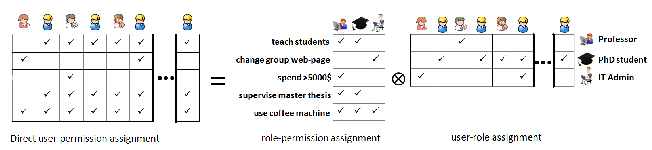
\includegraphics[width=\textwidth]{img/multi_assignment_rbac}
\end{figure}

\subsubsection{Evaluation Criteria}
For each role mining problem definition, there is a (set of) evaluation criteria:
\begin{itemize}
\item Matrix Reconstruction
\item Number of Sources
\item Inference Quality
\item Generalisation
\item Stability
\end{itemize}

\subsection{Binary Matrix Factorisation}
\emph{Min-Noise Approximation}: Given $K$, find the matrices $\hat U$, $\hat Z$ such that
\begin{align*}
    (\hat U, \hat Z) =\argmin_{U,Z} \norm{X-U\otimes Z}_1
\end{align*}
with $U\in \mathbb B^{D\times K}$ and $Z\in \mathbb B^{K\times N}$. This problem is also called \emph{approximate Boolean Matrix decomposition} and has the following properties:
\begin{itemize}
    \item \textbf{All} matrices are Boolean,
    \item It is a \emph{combinatorial optimisation problem},
    \item It is proven to be \emph{NP-hard} (reducible to set basis problem).
\end{itemize}
In contrast to recommender systems a the outputs $\hat U$ and $\hat Z$ are always binary.

\subsubsection{Rounded SVD}
\begin{enumerate}
    \item Compute the singular value decomposition
        \begin{align*}
            X=U\cdot S\cdot V^T
        \end{align*}
    \item Discard columns $K+1,\ldots,D$ of $U$ to get $U_{(K)}$.\\
          Discard rows $K+1,\ldots,N$ of $V$ to get $V_{(K)}$.
    \item Round the left and right singular vectors to get Boolean matrices $\hat U$ (roles) and $\hat Z$ (role assignments):
        \begin{align*}
            \hat U &= (U_{(K)} > t_U)\\
            \hat Z &= (V_{(K)} > t_V)
        \end{align*}
        where $t_U$ and $t_V$ are thresholds.
\end{enumerate}
The rounded continuous decomposition is a poor Boolean decomposition!

\subsubsection{$K$-means}
$K$-means partitions objects into disjoint groups (clusters) s.t. the average \emph{distance} between data and corresponding cluster prototypes is minimal. 
The standard objective function for $K$-means uses the \emph{Euclidean distance} measure:
\begin{align*}
    J(U,Z) = \norm{X-UZ}_2^2 = \sum_{n=1}^N \sum_{k=1}^K z_{kn} \norm{x_n - u_k}_2^2
\end{align*}
and centroids are updated via mean operation.

In order to use $K$-means for a Boolean decomposition the distance is adapted to use \emph{Hamming distance} (0-norm):
\begin{align*}
    J(U,Z) = \norm{X-UZ}_0 = \sum_{n=1}^N \sum_{k=1}^K z_{kn} \norm{x_n - u_k}_0
\end{align*}
The centroids $u_k$ are restricted to Boolean values and the centroid update step needs to be adapted:
\begin{align*}
    u_{dk} = \text{median}(\{x_{dn}|z_{kn} =1 \})\ \forall k\in \{1,\ldots,K\},\ \forall d \in \{1,\ldots, D\}
\end{align*}

$K$ can be found with cross-validation. $K$-means only yields \emph{disjoint clustering}, i.e. $Z$ matrix has only a single $1$ in each column. In RBAC however a user can have multiple role. 

\subsubsection{RoleMiner}
RoleMiner is a heuristic for role mining. Idea: A set of common permissions could potentially be a role. Roles are created by finding common sets of permissions between user.

Comes in two variants: \emph{CompleteMiner} and \emph{FastMiner}.

RoleMiner is very sensitive to noise:
\begin{itemize}
    \item If only a few individual bits are noisy, then the number of candidate roles gets much larger.
    \item The result is unstable: If the noise changes slightly, then the solution is completely different.
\end{itemize}

\subsubsection{DBPsolver}
DBPsolver approximately solves the \emph{Discrete Basis Problem}.
\paragraph{Discrete Basis Problem:} For a given Boolean matrix $X\in \mathcal B^{D\times N}$ and a number $K$ of basis vectors, find a Boolean matrix $U\in \mathcal B^{D\times K}$ and a Boolean matrix $Z\in \mathcal B^{K\times N}$ minimising 
\begin{align*}
    \norm{X-U\otimes Z}_F^2.
\end{align*}
The discrete basis problem and min-noise Role Mining problem are identical.

\subsubsection{Probabilistic Clustering}
\paragraph{Difficulties so far}
\begin{itemize}
 \item Searching in the full Boolean spaces has a \emph{too high complexity}.
 \item Restricting the Boolean search spaces \emph{ignores solutions}
 \item Searching solutions in continuous space and rounding \emph{produces poor results}.
 \item Search heuristics are prone to \emph{overfitting}
\end{itemize}

\paragraph{Modeling of RBAC} Computing a likelihood requires to design a probabilistic model $p(X|U,Z)$ for the generation process of the data $X$. This is the probability $X$ given the model, the cluster assignments $Z$, and the cluster centroids $U$.

\paragraph{Derivation I: One Object} For the simple case we consider one cluster per object:
\begin{align*}
\sum_k z_{kn} = 1, \qquad \forall n \in \{1, \ldots, N\}.
\end{align*}
$k_n$ is the cluster of object $n$: 
\begin{align*}
    k_{n} = \{ k\in \{1, \ldots, L\}| z_{kn} = 1\}.
\end{align*}
Consider on entry $x_{dn}$:\todo{WTF}
\begin{align*}
    p(x_{dn} = 0 | \beta_{d\cdot},z_{\cdot n}) = \beta_{dk_n}.
\end{align*}
Therefore:
\begin{align*}
    p(x_{dn} = 1 | \beta_{d\cdot},z_{\cdot n}) &=  1 - p(x_{dn} = 0 | \beta_{d\cdot},z_{\cdot n})\\
        &= 1-\beta_{dk_n}
\end{align*}

\paragraph{Derivation II: All objects} Objects are now independent given the parameters $Z$ and $U$. Thus:
\begin{align*}
    p(X|\beta,Z) &= \prod_{n=1}^N \prod_{d=1}^D p(x_{dn} = 1 | \beta_{d\cdot},z_{\cdot n})^{x_{dn}}\cdot p(x_{dn} = 0 | \beta_{d\cdot},z_{\cdot n})^{1-x_{dn}}\\
     &= \prod_{n,d} (1-\beta_{dk_n})^{x_{dn}} \beta_{dk_n}^{1-x_{dn}}
\end{align*}

\subsubsection{Multi-Assignment Clustering}
Compared to probabilistic clustering we don't restrict an object to one cluster.

One $x_{\cdot n}$ is generated by a \emph{set of clusters} $\mathcal L_n := \{k|z_{kn} = 1\}$. The resulting Boolean features are generated by \emph{disjunction} of the corresponding Boolean cluster centroids $u_{k,}$ (logical OR).
\begin{figure}[H]
    \centering
    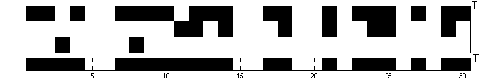
\includegraphics[width=0.8\textwidth]{img/multi_assignment_clustering}
    \caption{An object as the disjunction of the three clusters it belongs to.}
\end{figure}

\paragraph{Probabilistic view:} An object being generated by two clusters $k_1$, $k_2$ has probability $\beta_{dk_1}\beta_{dk_2}$ to have a $0$ at this dimension. 

Generally, an object $n$ belonging to the set of clusters $\mathcal L_n := \{ k|z_{kn} = 1\}$ has a probability $\beta_{\mathcal L_n} := \prod_{k\in \mathcal L_n} \beta_{dk}$ for a $0$ at dimension $d$.


In turn, it holds that $p(x_{dn}=1|z,\beta) = 1-\beta_{\mathcal L_n}$. Thus we get the following model:
\begin{align*}
    p(X|\beta, Z) = \prod_{n,d} \underbrace{\left(1-\prod_k \beta_{dk}^{z_{kn}} \right)^{x_{dn}} }_{\text{Noise component}} \underbrace{\left(\prod_k \beta_{dk}^{z_{kn}}\right)^{1-x_{dn}}}_{\text{Signal component}}
\end{align*}
\todo{Not sure about the component naming}

\subsubsection{Noise model for RBAC}

The deterministic RBAC generation of $X$:
\begin{align*}
    X = U\otimes Z \quad \Leftrightarrow\quad  x_{dn} = \bigvee_k [u_{dk} \land z_{kn}].
\end{align*}
Since this generation rule is not able to explain erroneous assignments in $X$ as noise we introduce a \emph{mixture noise model}:
\begin{align*}
    x_{dn} = (1-\xi_{dn})(U\otimes Z)_{dn} + \xi_{dn}\eta_{dn}
\end{align*}
where $\xi_{dn}$ is a binary noise indicator and $\eta_{dn}$ is a binary random variable.

\paragraph{Mixture Noise Model} Noise generation:
\begin{itemize}
    \item $\xi_{dn}$ indicates whether a bit is generated by $p_N (\xi_{dn}=1)$ or by $(U\otimes Z)_{dn}(\xi_{dn}=1)$. $\xi_{dn}$ is Bernoulli distributed:
    \begin{align*}
        p(\xi_{dn}|\varepsilon) = \varepsilon^{\xi_{dn}} (1-\varepsilon)^{1-\xi_{dn}},
    \end{align*}
    where $\varepsilon$ is the probability to choose a random bit.
    \item If the bits is noisy ($\xi_{dn}=1$), draw $\eta_{dn} = x_{dn}$ from
    \begin{align*}
        p_N(x_{dn}|r) = r^{x_{dn}} (1-r)^{1-x_{dn}},
    \end{align*}
    with $r$ being the probability that a noisy bit is $1$ ie. a user exceptionally gets a permission.
\end{itemize}
This can be modelled to a structure model:
\begin{align*}
    p_S(X|\beta, Z) = \prod_{n,d} \left( 1-\prod_k (\beta_{dk})^{z_{kn}}\right)^{x_{dn}} \left( \prod_k (\beta_{dk})^{z_{kn}}\right)^{1-x_{dn}},
\end{align*}
with $\beta_{dk}=p(u_{dk}=0)$.

This then can be combined with the noise model:
\begin{align*}
    p(X|Z, \beta, \xi, r) &= \prod_{n,d} p_N(x_{dn}|r)^{\xi_{dn}} p_S(x_{dn}|\beta_{d\cdot}, z_{\cdot n})^{1-\xi_{dn}}\\ 
    &= \prod_{n,d} \underbrace{\left( r^{x_{dn}}(1-r)^{1-x_{dn}}\right)^{\xi_{dn}}}_{x_{dn}\text{ generated by noise}}
    \underbrace{
        \left(\left[1-\prod_k (\beta_{dk})^{z_{kn}}\right]^{x_{dn}} 
            \left[ \prod_k(\beta_{dk})^{z_{kn}} \right]^{1-x_{dn}}
        \right)^{1-\xi_{dn}}
    }_{x_{dn}\text{ generated by roles}}.
\end{align*}

The $\xi_{dn}$ are unobservable (hidden) variables:
\begin{itemize}
\item They are unknown.
\item They are too many to be estimated.
\end{itemize}

We thus integrate the $\xi$ out of $p(X|Z,\beta, \varepsilon, \xi, r)$:
\begin{align*}
    p(X|Z,\beta,\varepsilon,r) = \sum_{\{\xi\}} p(X,\xi|Z,\beta, \varepsilon,r),
\end{align*}
where
\begin{align*}
    p(X,\xi|Z,\beta, \varepsilon, r) &=
        p(X|Z,\beta,\xi, r)p(\xi|\varepsilon)\\
        &= p(X|Z,\beta,\xi, r)\prod_{n,d}\varepsilon^{\xi_{dn}} (1-\varepsilon)^{1-\xi_{dn}}\\
        &= \prod_{n,d} \left(\varepsilon r^{x_{dn}} (1-r)^{1-x_{dn}}\right)^{\xi_{dn}}
            \left((1-\varepsilon)(1-\beta_{d,\mathcal L_n})^{x_{dn}}(\beta_{d,\mathcal L_n})^{1-x_{dn}}\right)^{1-\xi_{dn}}.
\end{align*}

\paragraph{Mixture Model:}
The likelihood function can thus be written as:
\begin{align*}
    p(X|Z,\beta,\varepsilon,r) &=
        \prod_{n,d} \left( \varepsilon r^{x_{dn}} (1-r)^{1-x_{dn}}+(1-\varepsilon)(1-\beta_{d,\mathcal L_n})^{x_{dn}} (\beta_{d,\mathcal L_n})^{1-x_{dn}} \right)\\
        &=  \prod_{n,d} \left(\varepsilon r + (1-\varepsilon)(1-\beta_{d,\mathcal L_n})\right)^{x_{dn}}
        \left(\varepsilon (1-r)+(1-\varepsilon)\beta_{d,\mathcal L_n}\right)^{1-x_{dn}}
\end{align*}
Parameters to estimate:
\begin{itemize}
    \item $Z$: user-role assignments.
    \item $\beta$: probabilities of role-permission assignments $U$ to be $0$.
    \item $\varepsilon$: noise probability.
    \item $r$: probability of noisy bits to be $1$.
\end{itemize}

This function requires a non-convex objective function to maximise the log-likelihood.
